\subsection{Operating Point and Static Characteristics}

To see the  non-linear  characteristics  of the plant, we set various constant
input voltages and waited for  the  motor  to  reach  its  settling speed. The
settling speed is then recorded and plotted in function of the  input  voltage
(see figure \ref{fig:static_cc}).

\begin{figure}[h]
    \centering
    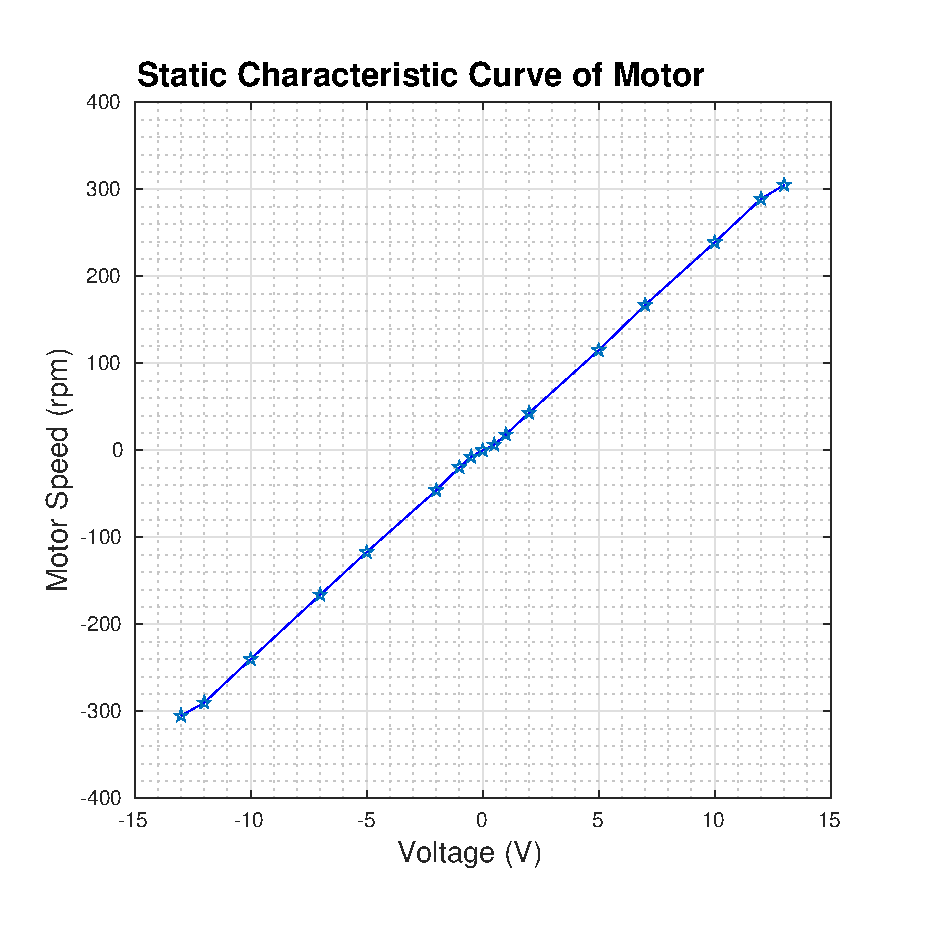
\includegraphics[width=\linewidth]{images/static_cc}
    \caption{Static characteristic curve of the plant (motor): Input voltage vs settling rotation speed.}
    \label{fig:static_cc}
\end{figure}

Of particular interest  are  the  areas  close  to \SI{0}{\volt} and the areas
close to  the  maximum  rotation  speed. This is where the plant is not at all
linear.

To see  how  these  non-linearities  affect the step response of the plant, we
performed  two  step  response  experiments,  one in the non-linear region  of
\SI{0}{\volt}-\SI{2}{\volt}  and  another  in  the  fairly  linear  region  of
\SI{2}{\volt}-\SI{10}{\volt}. The results of these experiments are recorded in
figure  \ref{fig:step_responses}  (left)  and   are  mapped  onto  the  static
characteristic curve (right).


When  comparing  the  input  amplitudes  of   both  steps  (\SI{2}{\volt}  and
\SI{8}{\volt}, respectively) to the  step  response  amplitudes  ($43$ rpm and
$197$ rpm, respectively), we expect a perfectly linear system  to  satisfy the
equation $\frac{43}{2} \stackrel{?}{=} \frac{197}{8}$, but this is clearly not
the case.

\begin{figure*}
    \centering
    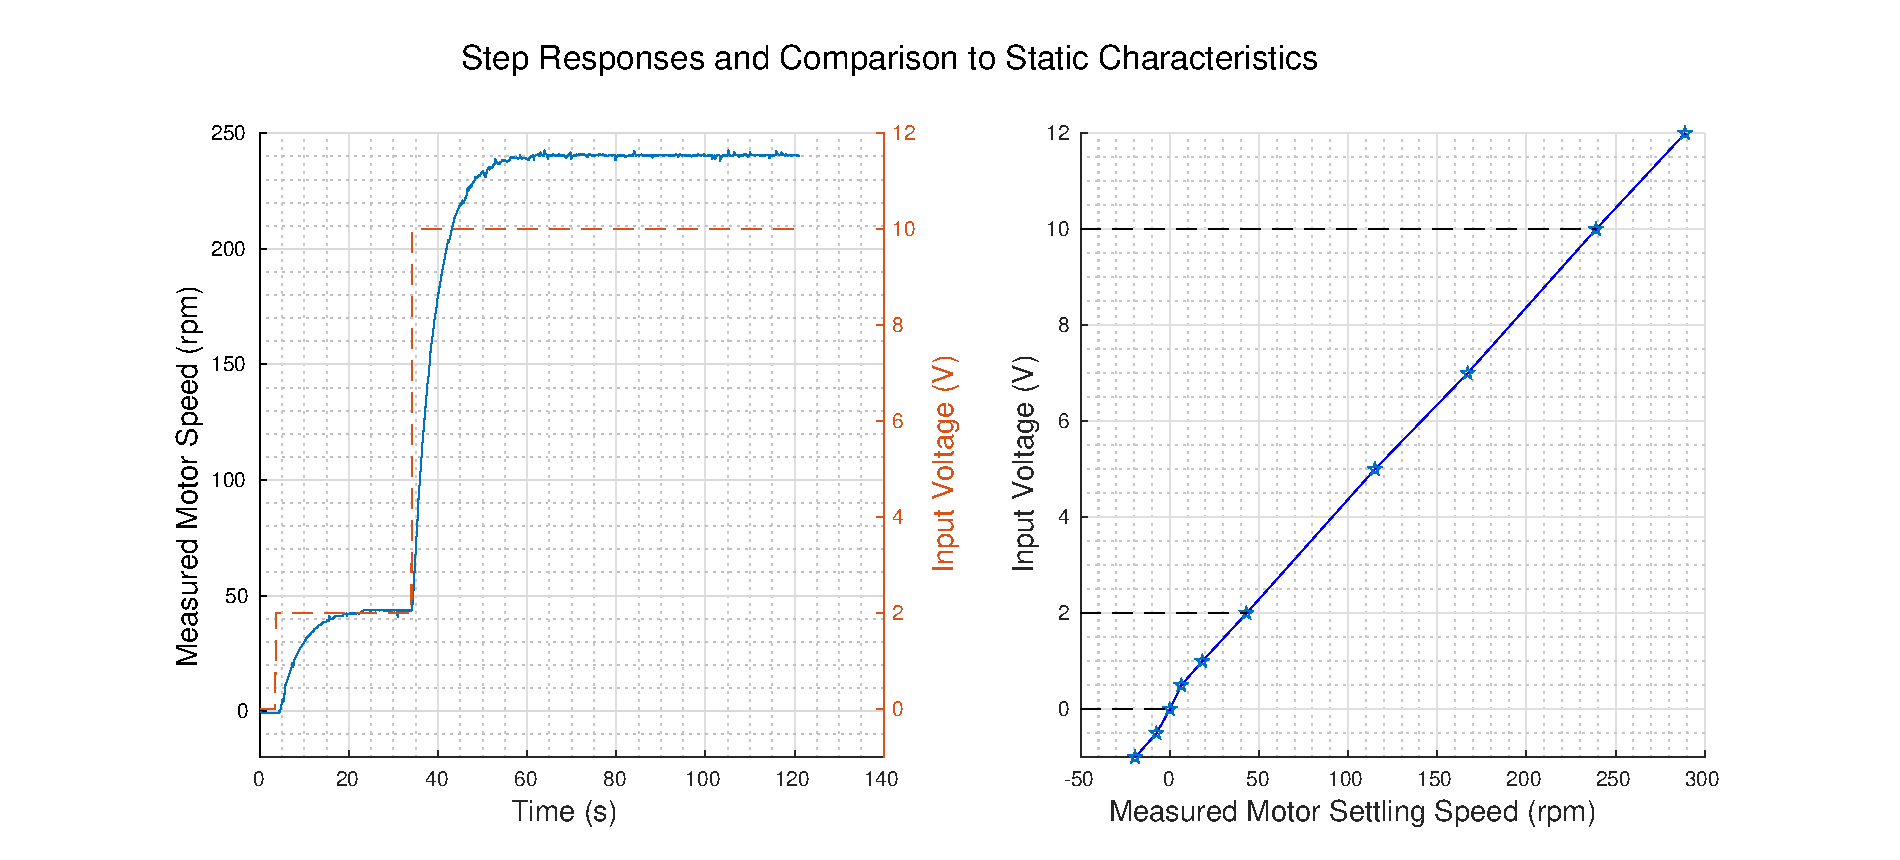
\includegraphics[width=\linewidth]{images/step_response}
    \caption{Two step response experiments, one in a non-linear region and the other in a fairly linear region. Notice how the step response amplitude differs between the two regions.}
    \label{fig:step_responses}
\end{figure*}

